% Source: graduate-coursework/Research/Intro_to_Agents/handouts/Part2_Agent_Foundations.tex

\documentclass[border=4pt]{standalone}
\usepackage{amsmath}
\usepackage{amssymb}
\usepackage{tikz}
\usepackage{xcolor}
\usetikzlibrary{shapes.geometric, arrows.meta, positioning, fit, calc, backgrounds}

\definecolor{UofSCGarnet}{HTML}{73000a}
\definecolor{UofSCBlack}{HTML}{000000}
\definecolor{UofSCWhite}{HTML}{ffffff}
\definecolor{UofSCAtlantic}{HTML}{466A9F}
\definecolor{UofSCCongaree}{HTML}{1F414D}
\definecolor{UofSCRose}{HTML}{CC2E40}
\definecolor{UofSCHorseshoe}{HTML}{65780B}
\definecolor{UofSCGrass}{HTML}{CED318}
\definecolor{UofSCHoneycomb}{HTML}{A49137}
\definecolor{UofSCDarkGarnet}{HTML}{570008}
\definecolor{UofSCAzalea}{HTML}{844247}
\definecolor{UofSC90Black}{HTML}{363636}
\definecolor{UofSC70Black}{HTML}{5C5C5C}
\definecolor{UofSC50Black}{HTML}{A2A2A2}
\definecolor{UofSCWarmGrey}{HTML}{676156}
\definecolor{UofSCSandstorm}{HTML}{FFF2E3}

\tikzset{
    % Box styles with sharp corners
    component/.style={
        rectangle,
        draw=UofSCBlack,
        fill=UofSCWhite,
        thick,
        minimum width=3cm,
        minimum height=1cm,
        align=center,
        font=\small
    },
    component garnet/.style={
        component,
        fill=UofSCGarnet!10,
        draw=UofSCGarnet,
        thick
    },
    component atlantic/.style={
        component,
        fill=UofSCAtlantic!10,
        draw=UofSCAtlantic,
        thick
    },
    component congaree/.style={
        component,
        fill=UofSCCongaree!10,
        draw=UofSCCongaree,
        thick
    },
    loop node/.style={
        rectangle,
        draw=UofSCGarnet,
        fill=UofSCGarnet!15,
        thick,
        minimum width=2.5cm,
        minimum height=1.2cm,
        align=center,
        font=\footnotesize\bfseries
    },
    decision/.style={
        diamond,
        draw=UofSCBlack,
        fill=UofSCHoneycomb!20,
        thick,
        minimum width=2cm,
        minimum height=1.5cm,
        align=center,
        font=\footnotesize,
        aspect=2
    },
    arrow style/.style={
        ->,
        >=Stealth,
        thick,
        UofSCBlack
    },
    biarrow style/.style={
        <->,
        >=Stealth,
        thick,
        UofSCBlack
    }
}

\begin{document}
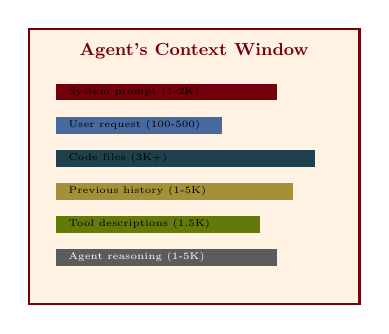
\begin{tikzpicture}[scale=0.7, transform shape]
                % Context window box
                \node[draw=UofSCGarnet, thick, minimum width=6cm, minimum height=5cm, fill=UofSCSandstorm] (window) at (0,0) {};
                \node[font=\small\bfseries, text=UofSCGarnet] at (0, 2.1) {Agent's Context Window};

                % Content bars
                \fill[UofSCGarnet] (-2.5, 1.5) rectangle (1.5, 1.2);
                \node[font=\tiny, anchor=west] at (-2.4, 1.35) {System prompt (1-2K)};

                \fill[UofSCAtlantic] (-2.5, 0.9) rectangle (0.5, 0.6);
                \node[font=\tiny, anchor=west] at (-2.4, 0.75) {User request (100-500)};

                \fill[UofSCCongaree] (-2.5, 0.3) rectangle (2.2, 0);
                \node[font=\tiny, anchor=west] at (-2.4, 0.15) {Code files (3K+)};

                \fill[UofSCHoneycomb] (-2.5, -0.3) rectangle (1.8, -0.6);
                \node[font=\tiny, anchor=west] at (-2.4, -0.45) {Previous history (1-5K)};

                \fill[UofSCHorseshoe] (-2.5, -0.9) rectangle (1.2, -1.2);
                \node[font=\tiny, anchor=west] at (-2.4, -1.05) {Tool descriptions (1.5K)};

                \fill[UofSC70Black] (-2.5, -1.5) rectangle (1.5, -1.8);
                \node[font=\tiny, anchor=west, text=white] at (-2.4, -1.65) {Agent reasoning (1-5K)};
            \end{tikzpicture}
\end{document}
